\section{Abstraction Relation between Path Conditions and Transformation Executions}
\label{sec:abstraction_relation}


% More informally, there exists a typed graph injective homomorphism between
% $Match_{pc}$ and $Input_x$  \textbf{and} $\langle V_x,E_x\setminus
% E_{mx},\tau_x\rangle$ is a typed graph strict instance of $\langle
% V_{pc},E_{pc}\setminus E_{pc},\tau_{pc}\rangle$.

% \levi{It is possible that this relation is required to be a typed graph strict
% instance between the path condition and the execution. Such a constraint would
% oblige each set of executions for a path condition to be truly distinct from
% the set of executions for another path condition. With the current definition
% the executions for a path condition including rule 'A' will overlap with the
% executions for a path condition including rules 'AB'. If this is so validity
% needs to be proved again for the new relation between the match patterns of PC
% and ex. Elements that do not show up in the match part of the rules are
% excluded from the typed graph strict instance.}



In this section we define the abstraction relation between the execution of a
DSLTrans transformation and the path condition that represents it.
This abstraction relation allows us to prove properties on a finite set of representative
path conditions, as created by the path condition generation algorithm. As this set is finite, our technique is  guaranteed to be decidable.

This section also presents our arguments that our path condition building
algorithm is both \emph{valid} and \emph{complete}. In this context
\emph{validity} means that for each path condition there exists at least one
transformation execution that it abstracts.
In other words, no path conditions are produced that lack a concrete
transformation execution counterpart. \emph{Completeness} of the symbolic
execution means that every transformation execution is abstracted by at least
one path condition.

Let us start by formally defining the notion of abstraction of a transformation
execution by a path condition.

\setcounter{equation}{0} 

\begin{definition}{Abstraction of a Transformation Execution by a Path Condition\\}
\label{def:abstraction_pc_ex}
\CatchFileBetweenTags{\abstractionrel}{text/definitions}{abstractionrel}{\abstractionrel}
\end{definition} 


% \cref{def:abstraction_pc_ex} enforces the fact that the matcher part of
% components of the path condition are found through an injective typed graph
% homomorphism in the execution's input model. Additionally, the graph including
% the output of the execution (including traceability information), can be
% mapped by a surjective typed graph homomorphism onto the apply model (plus the
% symbolic traceability links) of the path condition.

To understand the abstraction relation in \cref{def:abstraction_pc_ex}, recall
that during the construction of a transformation execution rules are matched
injectively in the input model. This information is present in the first
condition of the abstraction relation (Proposition~\ref{eq:abstr_input_output})
via the injective typed graph homomorphism between the match part of the copies
of rules ``glued'' onto the path condition and the containment transitive
closure of the input part of the transformation execution. This relation
enforces the fact that certain parts of the execution were found, or matched, by
certain parts of the path condition.
On the other hand, the surjection from the output of the execution towards the
apply part of the path condition models the fact that the output of the
execution has been completely built by instantiating the apply parts of the
rules contained in the path condition.

The second condition of the abstraction relation
(Proposition~\ref{eq:abstr_trace}) checks for the fact that symbolic
traceability links in the path condition and traceability links in the execution
correctly correspond to each other. This is modeled by the fact that all
strongly connected components in the path condition, composed only of symbolic
traceability links, are injectively found on the execution. This injection
models the fact that traceability graphs between individual or combined rules in
the path condition are necessarily found in the execution. Note that components
of the path condition are considered because of the fact that disconnected rules
in the path condition may have matched over common elements of a particular
execution. As such, a full injection between the complete traceability graph in
the path condition and the execution would be incorrect. Additionally, in the
second part of Proposition~\ref{eq:abstr_trace} we check the fact that every
traceability link in the execution can be found in the path condition. This
additional sanity check enforces that no spurious traceability links that could
not have been created by the rules present in the path condition exist in the
transformation execution.

%Finally, the last clause of the abstraction relation states that rule copies
%that are repeated a number of times in the path condition need to be found at
%least a similar amount of times in the abstracted transformation execution.

It is important to mention that another abstraction relation, weaker or
stronger, could have been chosen. The abstraction relation presented in
\cref{def:abstraction_pc_ex} suits our needs in the sense that it allows us to
demonstrate the validity and completeness of our proof technique, as we will
show in the text follows. Additionally, it is particularly interesting because
it makes sure that, given a DSLTrans transformation, each of its transformation
executions is abstracted by one and only one of its path conditions. This result
adds to the consistency of our theory and is also exposed later in this section.



\subsection{Examples}

In this section, we provide a number of examples to demonstrate the workings of
the abstraction relation we chose to use. \cref{fig:legend} presents the legend
for the following figures.

\begin{figure}[htb]
 \centering
                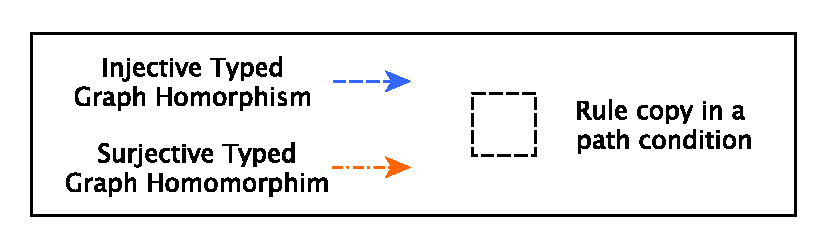
\includegraphics[width=0.5\textwidth]{./figures/abstraction_relation/legend.pdf}
                \caption{Legend for abstraction relation figures}
                \label{fig:legend}
\end{figure}
                
\subsubsection{Example 1 -- Empty Path Condition}

We begin by defining which transformation executions an empty path condition
will abstract. \cref{fig:empty_pc} demonstrates two cases. In each, the path
condition \textit{pc} is on the left-hand side, and a transformation execution \textit{ex} is on the
right-hand side. Note that in \cref{fig:empty_pc_success}, the path condition
abstracts the transformation execution, while in \cref{fig:empty_pc_fail}, the
abstraction relation does not hold.

\begin{figure}[htb]
        \centering
        \begin{subfigure}[b]{0.40\textwidth}
                \centering
                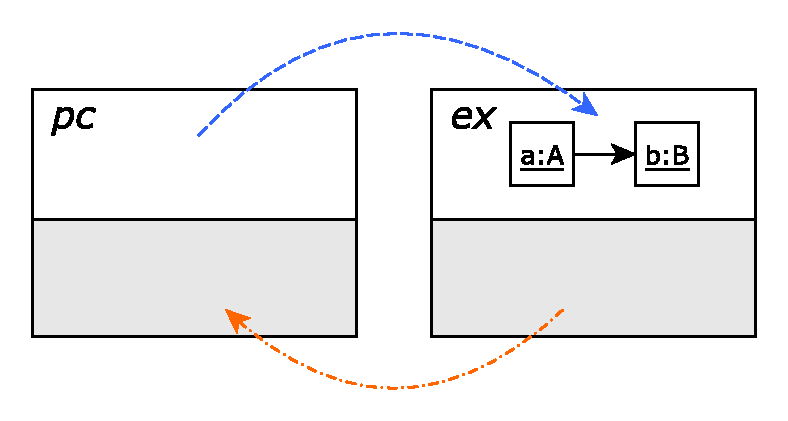
\includegraphics[width=1\textwidth]{./figures/abstraction_relation/empty_pc.pdf}
               	\caption{Abstraction holds}
               	\label{fig:empty_pc_success}
        \end{subfigure}%
        ~~\\
        \begin{subfigure}[b]{0.40\textwidth}
                \centering
                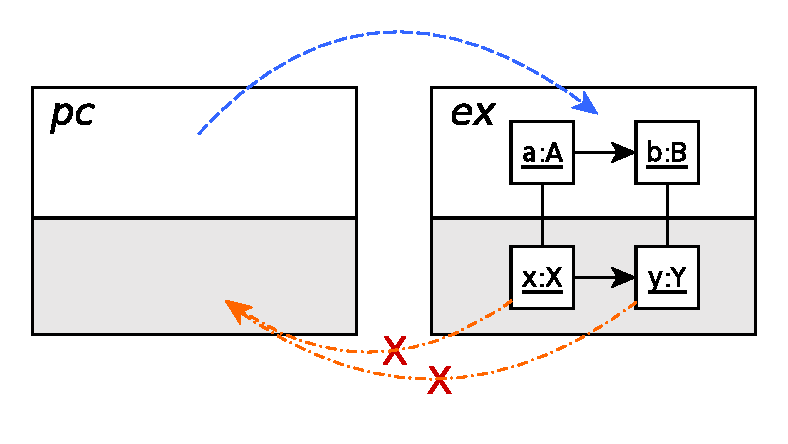
\includegraphics[width=1\textwidth]{./figures/abstraction_relation/empty_pc2.pdf}
                \caption{Abstraction does not hold}
                \label{fig:empty_pc_fail}
        \end{subfigure}%
        \caption{Abstraction of transformation executions by the empty path condition}
        \label{fig:empty_pc}
\end{figure}


The match part of the path condition represents the pre-conditions for the path condition to be true, depending on which rules have symbolically executed in the transformation. For example, if the match graph is empty, this represents all executions where no rules have executed. 

The first condition for the abstraction relation is to determine whether a typed graph injective homomorphism can be found between the match graph of the path condition, and a transformation execution. Note that in both \cref{fig:empty_pc_success} and \cref{fig:empty_pc_fail}, an empty typed graph homomorphism satisfies this condition, highlighted by blue arrows.


The second condition for the abstraction relation is whether a typed graph surjective homomorphism can be found from the transformation execution's output model to the apply graph of the path condition. This is represented by orange arrows in \cref{fig:empty_pc_success} and \cref{fig:empty_pc_fail}. This relation is surjective as there may not be any elements in the output model that are not represented by the path condition's apply graph. Note that multiple elements in the output model may match to the same element in the apply graph of the path condition. This is expected, as the structure found in the apply graph may be found multiple times in the output model.


The empty apply graph of the path condition defines no post-conditions on the output model, as no rules have executed. Note that there an empty surjective typed graph homomorphism can be found between the output model of the transformation execution in \cref{fig:empty_pc_success} and the path condition. This is intuitive, as the lack of elements in the output model means no rules have executed, which corresponds to the lack of post-conditions defined by the path condition.


In contrast, there is no surjection between the elements of the output model in \cref{fig:empty_pc_fail} and the path condition. Note that the transformation execution has elements in the output model and thus at least one rule must have executed. However, the path condition does not represent that a rule has executed. Therefore, the path condition shown does not represent this execution. 

%The fact that this transformation execution will be abstracted by at least one path condition is demonstrated by \cref{prop:pc_completeness}.



\subsubsection{Example 2 -- Non-overlapping Rule Components}


This second example shows the abstraction relation between path conditions and transformation executions, when no match element of the same type appears in multiple rule components.

For these examples, we will represent the abstraction relation with two figures. The first will demonstrate the matching performed on match and apply graphs, while the second figure focuses on traceability link matching.

Let us first examine how the injection operates between the match elements in the path condition and the transformation executions in \cref{fig:non_overlapping_match_apply} and \cref{fig:non_overlapping2_match_apply}. Note that this injection can be found in both cases.

\begin{figure}[htb]
        \centering
        \begin{subfigure}[b]{0.40\textwidth}
                \centering
                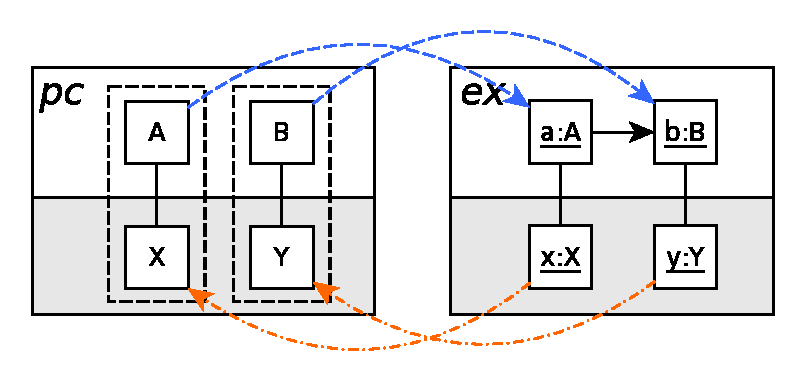
\includegraphics[width=1\textwidth]{./figures/abstraction_relation/non_overlapping.pdf}
               	\caption{Abstraction holds on match and apply graphs}
               	\label{fig:non_overlapping_match_apply}
        \end{subfigure}%
        ~~\\
        \begin{subfigure}[b]{0.40\textwidth}
                \centering
                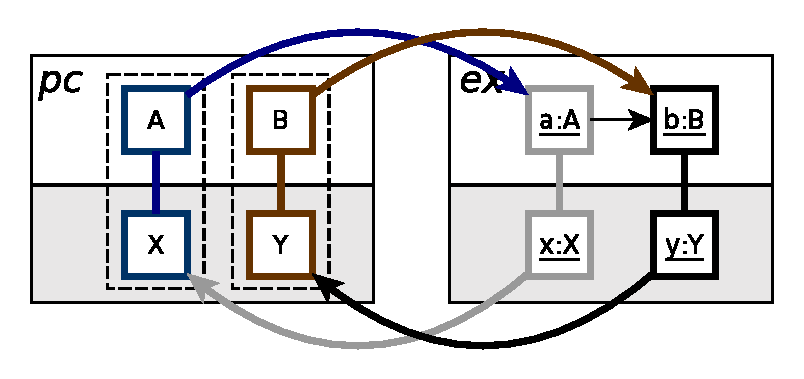
\includegraphics[width=1\textwidth]{./figures/abstraction_relation/non_overlapping_trace_links.pdf}
                \caption{Abstraction holds on traceability links}
                \label{fig:non_overlapping_trace_links}
        \end{subfigure}%
        \caption{Abstraction of transformation execution by non-overlapping rule components}
        \label{fig:non_overlapping}
\end{figure}


\begin{figure}[htb]
        \centering
        \begin{subfigure}[b]{0.40\textwidth}
                \centering
                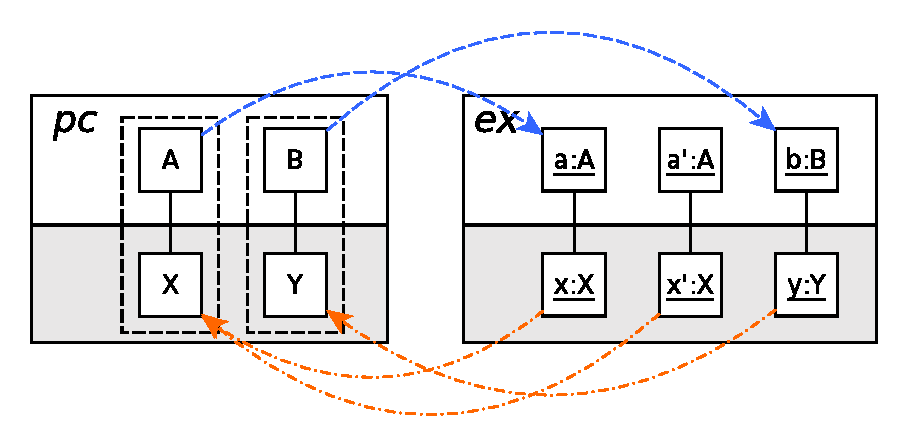
\includegraphics[width=1\textwidth]{./figures/abstraction_relation/non_overlapping2.pdf}
               	\caption{Abstraction holds on match and apply graphs}
               	\label{fig:non_overlapping2_match_apply}
        \end{subfigure}%
        ~~\\
        \begin{subfigure}[b]{0.40\textwidth}
                \centering
                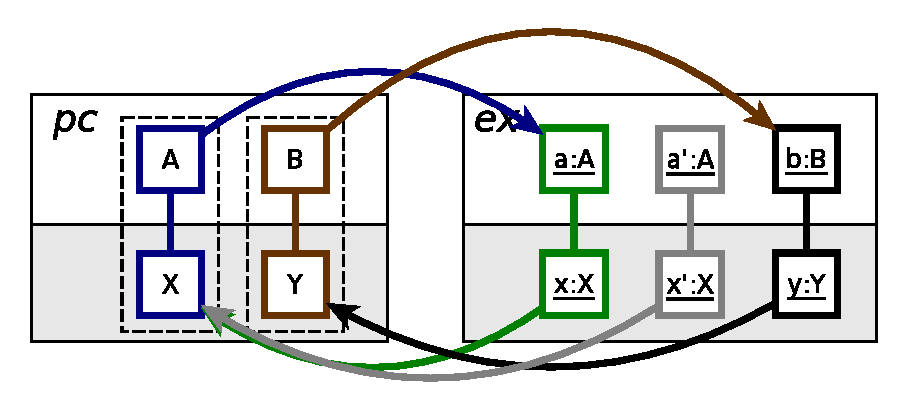
\includegraphics[width=1\textwidth]{./figures/abstraction_relation/non_overlapping2_trace_links.pdf}
                \caption{Abstraction holds on traceability links}
                \label{fig:non_overlapping2_trace_links}
        \end{subfigure}%
        \caption{Example of abstraction over multiple rule execution}
        \label{fig:non_overlapping2}
\end{figure}

Similarly, there is a surjection between the elements of the output model for both transformation execution and the apply graph of the respective path condition. Note that this surjective match also holds in \cref{fig:non_overlapping2_match_apply}, where examination of the transformation execution shows that one rule has executed twice. As mentioned before, the abstraction relation abstracts over the number of times that a rule has executed.

We also note that these matches must also match over associations between the elements, including association typing. This is not included in the figures for visual clarity.


We now examine \cref{fig:non_overlapping_trace_links} and \cref{fig:non_overlapping2_trace_links} to resolve whether the traceability links in the path condition can be found in the transformation execution. This matching is represented by the arrows from each component highlighted in a bold outline and differentiated by colour. We note that each component in the path condition can be successfully found in the transformation execution.

As well, there is a matching step from each individual traceability link in the transformation execution onto the path condition. Similar to the matching from the path condition, the bold components in the transformation execution figure are matched onto the path condition. We note that this matching is successful as well.


\subsubsection{Example 3 -- Overlapping Rule Components}
\label{subsubsec:abstraction_relation_overlapping}

For these examples, the path conditions contain overlapping rule components, i.e. separate rules share match elements of the same type. Our goal is to illustrate the interaction of rule elements, where the elements of non-dependent rules may match over the same or different elements in the transformation execution.

For example, the two rule components in \cref{fig:overlapping_match_apply} correctly match over the transformation execution shown. The abstraction relation holds due to the fact that, while match elements of the same component need to be found injectively in the execution, the injection constraint does not span multiple components. This allows the match elements from different rules to match to the same input model element.


\begin{figure}[htb]
        \centering
        \begin{subfigure}[b]{0.40\textwidth}
                \centering
                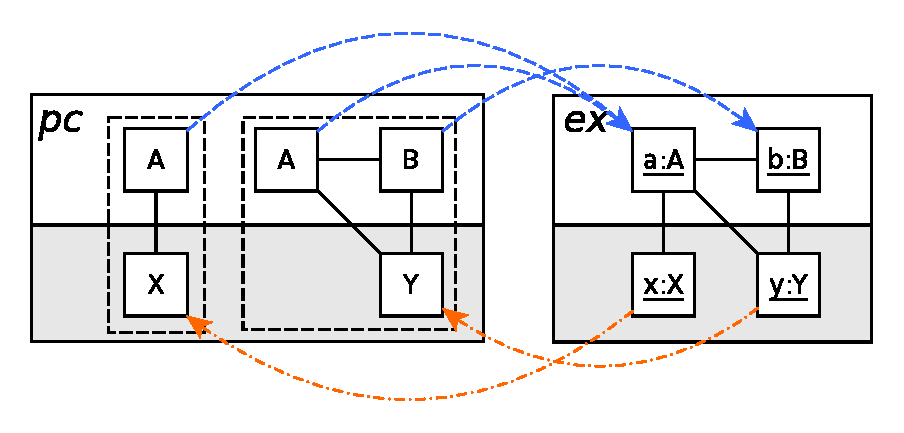
\includegraphics[width=1\textwidth]{./figures/abstraction_relation/overlapping.pdf}
               	\caption{Abstraction holds on match and apply graphs}
               	\label{fig:overlapping_match_apply}
        \end{subfigure}%
        ~~\\
        \begin{subfigure}[b]{0.40\textwidth}
                \centering
                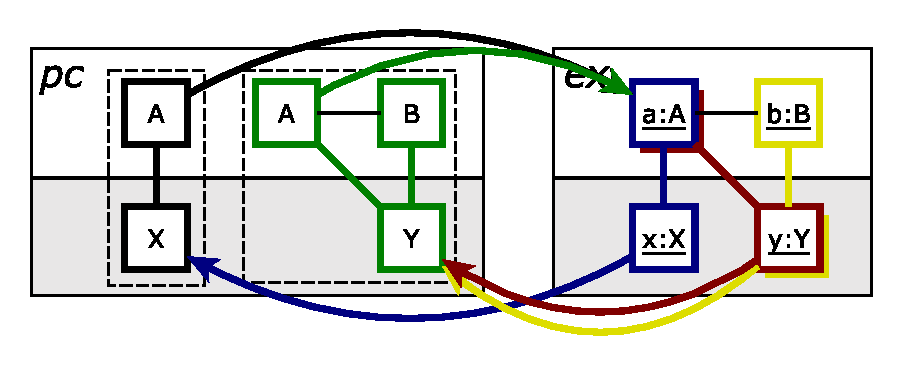
\includegraphics[width=1\textwidth]{./figures/abstraction_relation/overlapping_trace_links.pdf}
                \caption{Abstraction holds on traceability links}
                \label{fig:overlapping_trace_links}
        \end{subfigure}%
        \caption{Abstraction of transformation execution by overlapping rule components}
        \label{fig:overlapping}
\end{figure}

As well, \cref{fig:overlapping_trace_links} shows the mapping from the path condition to the transformation execution. However, note that the pattern composed of the A, B, and Y elements, along with the traceability links, is to be matched as a whole. This is to ensure that the traceability links are found in the proper configuration in the transformation execution.

We also match the traceability links from the transformation execution back onto the path condition. Again, this is to ensure that no traceability links are found in the transformation execution that have not been represented in the path condition. Three matches are performed in this step, denoted by the three arrows in the bottom of \cref{fig:overlapping_trace_links}. Each match is composed of a traceability link as well as immediately connected elements.

\begin{figure}[htb]
        \centering
        \begin{subfigure}[b]{0.40\textwidth}
                \centering
                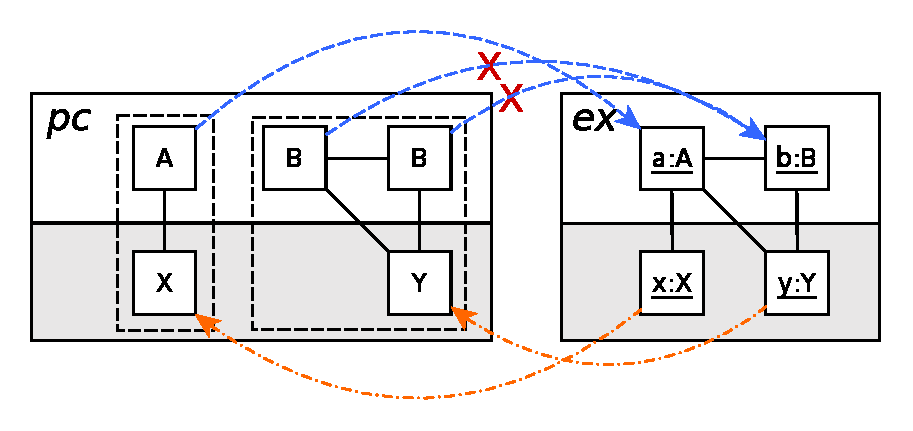
\includegraphics[width=1\textwidth]{./figures/abstraction_relation/overlapping2.pdf}
               	\caption{Elements cannot overlap within a component}
               	\label{fig:overlapping2_match_apply}
        \end{subfigure}%
        ~~\\
        \begin{subfigure}[b]{0.40\textwidth}
                \centering
                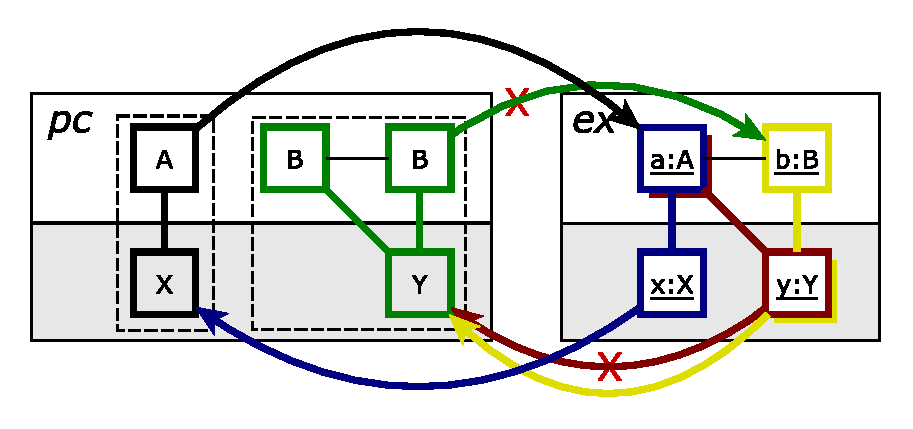
\includegraphics[width=1\textwidth]{./figures/abstraction_relation/overlapping2_trace_links.pdf}
                \caption{Traceability links cannot be found}
                \label{fig:overlapping2_trace_links}
        \end{subfigure}%
        \caption{Abstraction does not hold}
        \label{fig:overlapping2}
\end{figure}


In contrast to \cref{fig:overlapping}, \cref{fig:overlapping2} shows an example where the abstraction relation does not hold. Consider \cref{fig:overlapping2_match_apply}. Note that a component in the match graph of the path condition contains two B elements. Both of these elements must be found in the transformation execution, and thus it is not correct for them to injectively match to the same element in the input model.

As well, it is informative to examine \cref{fig:overlapping2_trace_links}. Note the one of the matches from the transformation execution attempts to match over 'a:A' and 'y:Y' elements, connected by a traceability link. Examination of the path condition shows that this traceability link is not present. Therefore, this path condition cannot accurately represent this transformation execution.


\subsubsection{Example 4 -- Indirect Links}

\begin{figure}[htb]
        \centering
        \begin{subfigure}[b]{0.40\textwidth}
                \centering
                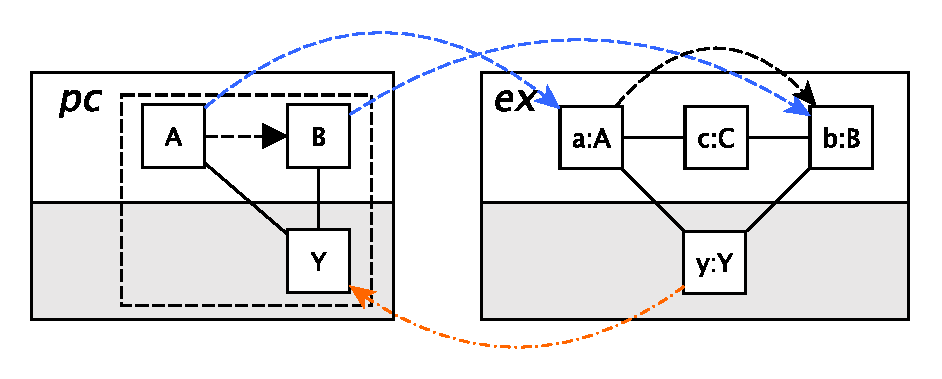
\includegraphics[width=1\textwidth]{./figures/abstraction_relation/indirect.pdf}
               	\caption{Matching over match and apply graphs}
               	\label{fig:indirect_match_apply}
        \end{subfigure}%
        ~~\\
        \begin{subfigure}[b]{0.40\textwidth}
                \centering
                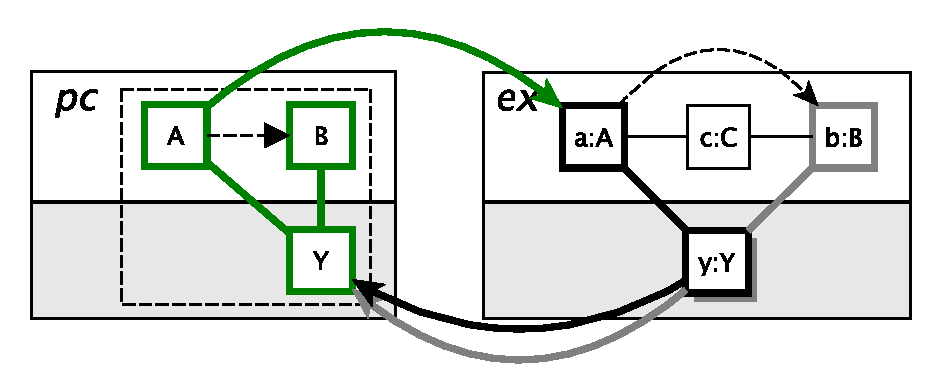
\includegraphics[width=1\textwidth]{./figures/abstraction_relation/indirect_trace_links.pdf}
                \caption{Matching over traceability links}
                \label{fig:indirect_trace_links}
        \end{subfigure}%
        \caption{Abstraction with indirect links}
        \label{fig:indirect}
\end{figure}

\begin{figure*}[htb]
        \centering
        \begin{subfigure}[b]{0.70\textwidth}
                \centering
                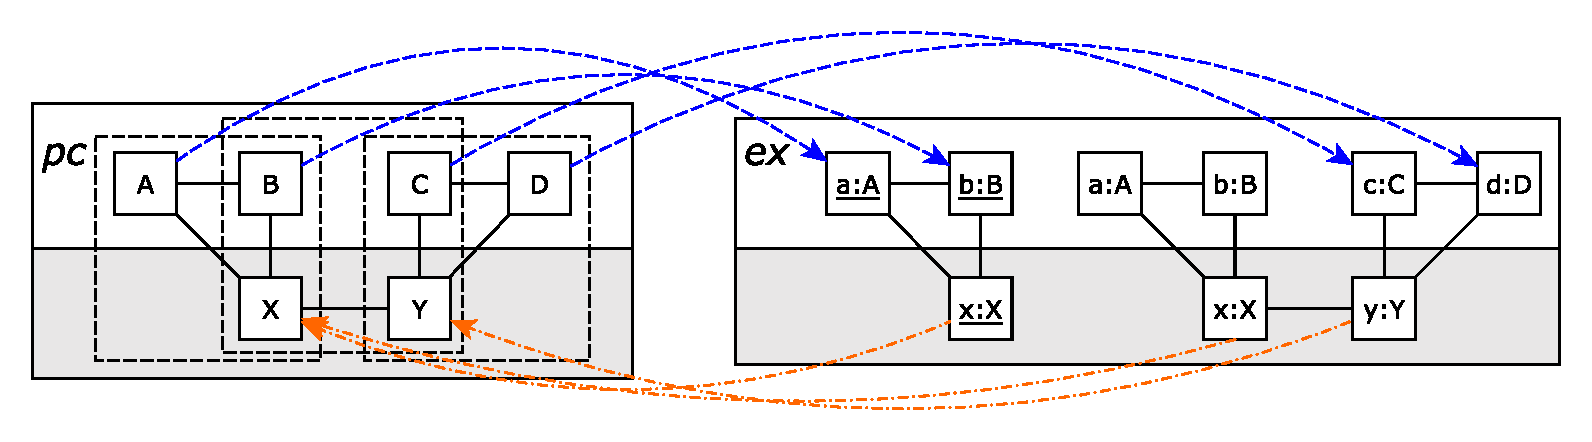
\includegraphics[width=1\textwidth]{./figures/abstraction_relation/combination.pdf}
               	\caption{Abstraction holds on match and apply graphs}
               	\label{fig:combination_match_apply}
        \end{subfigure}%
        ~~\\
        \begin{subfigure}[b]{0.70\textwidth}
                \centering
                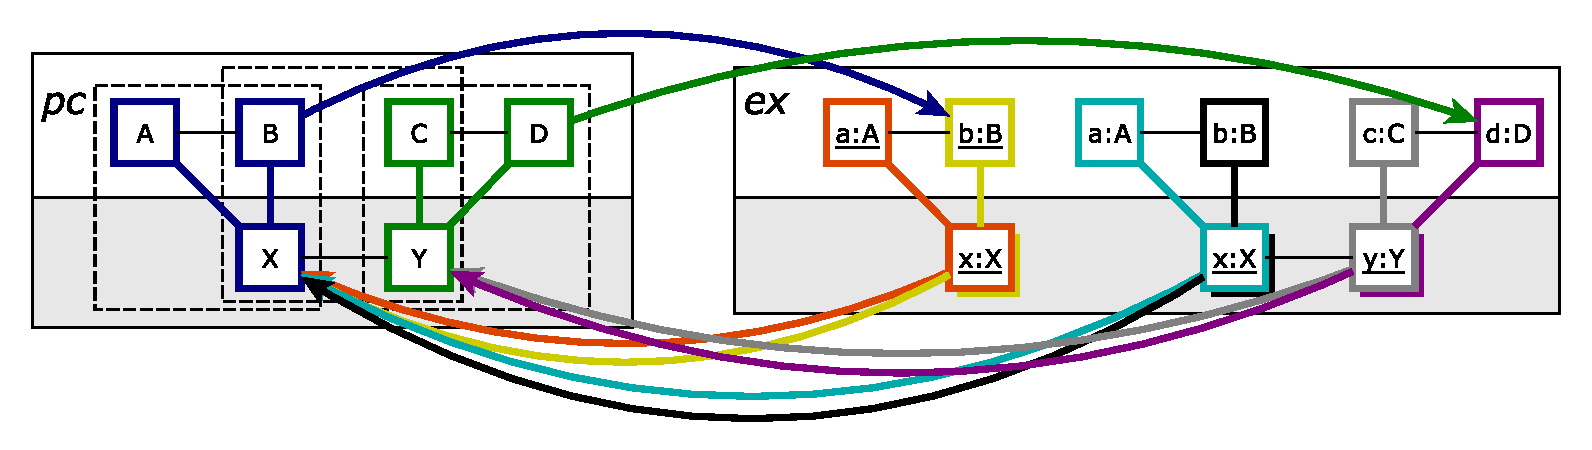
\includegraphics[width=1\textwidth]{./figures/abstraction_relation/combination_trace_links.pdf}
                \caption{Abstraction holds on traceability links}
                \label{fig:combination_trace_links}
        \end{subfigure}%
        \caption{Abstraction where path condition has combined rules}
        \label{fig:combination}
\end{figure*}

We now present a path condition  in \cref{fig:indirect_match_apply} that includes indirect links. In this case, for the injective match to hold, the elements at both ends of the link must be found, and there must be an indirect link between the matched elements and between the elements in the transformation execution.

Note that the indirect link between elements $a:A$ and $b:B$ in the transformation execution is added by the containment transitive closure $Input^{*}$ in proposition~\ref{eq:abstr_input_output} of \cref{def:abstraction_pc_ex} to allow matching indirect links. Note also that, for the sake of our example, we are assuming that the links between $a:A$, $b:b$ and $c:C$ are containment relations.

\cref{fig:indirect_trace_links} highlights the structures involved in matching over traceability links. From the path condition, the structure contains the A, B, and Y elements with connected traceability links. From the transformation execution, there are two structures to be found in the path condition denoted in bold in the transformation execution. The matching of all structures can be successfully performed, and thus this abstraction relation holds.


%Note that only the match graph of the path condition may include an indirect link.



\subsubsection{Example 5 -- Combined Rules}



\cref{fig:combination} shows a path condition that is composed of a multitude of rules which have been combined in the path condition generation algorithm. Each individual rule is surrounded by dashed lines.

Note that the matching on the match and apply graphs in \cref{fig:combination_match_apply} is similar to other examples. The combined rules can be considered as a single graph for the abstraction relation.

\cref{fig:combination_trace_links} shows the matching when multiple traceability links are present in the transformation execution. Note that each individual traceability link and the connected elements are matched onto the path condition.

\subsection{Validity and Completeness}
\label{subsec:abstraction_relation_validity_completeness}

In this section, we discuss the validity and completeness of the abstraction relation. Only proof sketches are presented here for \cref{prop:pc_validity} and \cref{lem:uniqueness}, while more complete proofs are found in \cref{sec:val_complete_path_cond_gen}, in the proofs of \cref{prop:pc_validity_appendix} and \cref{lem:uniqueness_appendix} respectively.


%\newpage
\begin{proposition}{(Validity)}
\label{prop:pc_validity}
Every path condition abstracts at least one transformation execution.
\end{proposition}
\begin{ps}

Let $tr\in \textsc{Transf}^{sr}_{tg}$ be a DSLTans transformation. We wish to demonstrate that, for all path conditions $pc\in \textsc{Pathcond}(tr)$, there exists a transformation execution $ex\in \textsc{Exec}(tr)$ of the set of
rules used to build $pc$ such that $pc$ abstracts $ex$, as formally expressed in \cref{def:abstraction_pc_ex}. We can prove this property by induction on the set of transformations $\textsc{Transf}^{sr}_{tg}$ (see \cref{def:layer_transformation}), as follows:

\begin{itemize}
  \item \emph{Base case:} the base case is when $tr$ is the empty
  transformation. In this case, according to \cref{def:path_cond_gen} only the
  empty path condition $\epsilon_{pc}$ exists in the path condition set. We thus
  need to demonstrate that the empty path condition abstracts the empty
  transformation execution $\epsilon_{ex}$, as well as any execution for which
  the input model is never matched by any rule (consequently having an empty
  output model). For any of these transformation executions, Proposition~\ref{eq:abstr_input_output} of the abstraction relation definition is satisfied, as no rule copy exists in the path condition and the output of the transformation execution is empty -- empty typed graph homomorphisms thus satisfy all the conditions of the proposition. Proposition~\ref{eq:abstr_trace} of the abstraction relation definition also trivially holds because no traceability links exist either in the path condition or in any of the considered executions.
  
%   This is so because:
%   1) the empty typed graph homomorphism is an injective typed graph homomorphism
%   between the match part of the empty path condition and any input model; and 2) as
%   well as a surjective typed graph homomorphism between an empty output model
%   and the apply part of the empty path condition.
 
\item \emph{Inductive case:} assuming every path condition generated for a transformation $tr$ abstracts at least one transformation execution, we need to show that every path condition generated for a transformation $tr'$, resulting from adding a layer $l\in \textsc{Layer}^{sr}_{tg}$ to $tr$, will also abstract at least one transformation execution. 
\end{itemize}

In order to demonstrate the inductive case we need to show the property holds for all path conditions resulting from combining the rules of layer $l$ with any path condition generated for $tr$. These path conditions for transformation $tr'$ are built as expressed in \cref{def:path_cond_layer_comb}. According to this definition, path conditions for $tr'$ are built by incrementally combining the path conditions generated for $tr$ with a rule of layer $l$, until all the rules in $l$ have been treated. We can thus again use induction for this proof, this time on the set of possible layers $\textsc{Layer}^{sr}_{tg}$. 

\begin{itemize}
  \item \emph{Base case:} this is the case where layer $l$ contains no rules. In this case, by the base case of \cref{def:path_cond_layer_comb}, no new path condition is added to the set of path conditions generated for the transformation $tr$. As such the $tr=tr'$ and by induction hypothesis the property trivially holds for all path conditions generated for $tr'$.
  
  \item \emph{Inductive case:} for the inductive case (transitive case of \cref{def:path_cond_layer_comb}) we need to show that, assuming the property holds for all path conditions generated for a transformation $tr$, then the property will also hold for a transformation $tr'$ -- where $tr'$ results from adding a new rule $rl$ to the last layer of $tr$. We will thus need to consider the four \reviewer{three?} cases of rule combination:\vspace{.2cm} 
 
\begin{enumerate}
\item\label{lab:rule_case1} Rule $rl$ has no dependencies (\cref{def:rule_comb_no_dependencies}).
\item\label{lab:rule_case2} Rule $rl$ has dependencies and cannot execute (\cref{def:rule_comb_unsatisfied}).
\item\label{lab:rule_case3} Rule $rl$ has dependencies and may and/or will execute (\cref{def:rul_comb_partial_total}).
\end{enumerate}

The property trivially holds for case~\ref{lab:rule_case2}, given that no new path conditions are added to the path condition set generated for $tr$ and that the property holds for $tr$ by induction hypothesis. When a rule $rl$ is added to the last layer of $tr$ such that cases~\ref{lab:rule_case1} or~\ref{lab:rule_case3} occur, then the property can be shown to hold for $tr'$ as follows: 1) choose for a general path condition $pc$ generated for $tr$ an execution $ex$ such that $pc$ abstracts $ex$; 2) build an input model $m$ as the result of uniting the input model of $ex$ with a model that can be matched by $rl$; 3) execute $tr'$ having as input model $m$ to produce transformation execution $ex'$; and finally 4) demonstrate $ex'$ is abstracted by the path condition $pc'$ resulting from combining $pc$ with $rl$ whether rule $rl$ does not depend on $pc$ or rule $rl$ depends on $pc$ and may and/or will execute.
\end{itemize}
\end{ps} 


\begin{proposition}{(Completeness)}
\label{prop:pc_completeness}
Every transformation execution is abstracted by one path condition.
\end{proposition}
\CatchFileBetweenTags{\pathgencompletenessproof}{text/definitions}{pathgencompletenessproof}{\pathgencompletenessproof} 

% Our path conditions construction algorithm takes all possible interactions of rules
% into account:
% \begin{enumerate}
% \item When building the path conditions for one layer we have built all
% the combinations of rules, as well as their possible interactions through
% \emph{disambiguation};
% \item When combining the path conditions from different layer different layers
% we have considered the cases where no interactions exist, or where backward
% links in rules requires certain certain elements to already exist in the
% generated model thus far.
% \end{enumerate}
% Note that, given the considered subset of DSLTrans constructs as described
% in \cref{sec:dsltrans}, no additional cases of rule interaction other than the
% ones described above need to be considered.
% From \cref{prop:pc_validity} we also know that at least one concrete
% transformation execution exists per path condition. In the proof of
% \cref{prop:pc_validity} we have built, for each path condition $A$,
% the simplest transformation execution that is abstracted by $A$. These
% transformation executions produce one instance of each element and association
% present in the apply pattern of $A$. However, given
% \cref{def:instance_pc_ex} in \cref{sec:proofs} (abstraction of
% a transformation execution by a path condition), an infinite amount of
% transformation executions are always abstracted by $A$. These executions
% correspond to the generation of output models holding an arbitrarily large
% amount of the elements and associations while still being abstracted by $A$.
% Because we have considered all possibilities of execution in our path condition
% construction algorithm, the union of all transformation executions built for
% each path condition constitutes the complete, infinite set of transformation
% executions. We thus know that every possible transformation execution is
% abstracted by at least one path condition.


% Note that we do not provide any guarantee that the same transformation execution
% cannot be abstracted by two different path conditions. Although given our symbolic
% execution assumptions we believe this to be the case, further mathematical
% exploration of this issue is necessary. Given however the fact that our
% verification algorithm exhaustively explores all path conditions, it is
% sufficient for the property proof to provide a \emph{no} result in the analysis
% of a path condition for the result of the verification of the property to be
% \emph{no}. \levi{keep this?}

\begin{lemma} (Uniqueness) 
\label{lem:uniqueness}
A transformation execution is abstracted by exactly one path condition.
\end{lemma}
\begin{ps}
Let $tr\in \textsc{Transf}^{sr}_{tr}$ be a model transformation. We will demonstrate that two different path conditions\\$pc_1, pc_2\in \textsc{Pathcond}(tr)$ cannot exist such that we have a transformation execution $ex\in \textsc{Exec}(tr)$ where $ex\Vvdash pc_1$ and $ex\Vvdash pc_2$.

We will do so by attempting to build an $ex\in \textsc{Exec}(tr)$ such that $ex\Vvdash pc_1$ and $ex\Vvdash pc_2$ and demonstrating that it is always the case that such is not possible. In order to structure our argumentation, we will consider two cases:
% \levi{the contradiction happens because at each point of the execution, when a rule is added any two path conditions from the existing set of path conditions will represent different executions. At all points if we consider two path conditions in the PC set we have that two different executions can be created if we find a model that satisfies the first condition of the abstraction relation, and it is always the case that none of those two executions can be abstracted by the two path conditions simultaneously.}
\begin{enumerate}
  \item\label{item:uniqueness_rule_no_dep} the case where no rules in $tr$ have dependencies.
  \item\label{item:uniqueness_rule_has_dep} the case where some rules in $tr$ have dependencies.
\end{enumerate}

We start by considering that $tr$ falls into case~\ref{item:uniqueness_rule_no_dep} above. By~\cref{def:path_cond_gen} of path condition generation, each rule appears at most once in a path condition. Also, by construction, each path condition always contains a different combination of rules. We additionally know from \cref{def:layer_transformation} that the rules that compose $tr$ necessarily have non-overlapping matchers. We can nonetheless build a model $m$ as the typed graph union of two input models $m_1$ and $m_2$, where injective typed graph morphisms can be found between the match parts of the rule copies that form $pc_1$, and $m_1$. Injective typed graph morphisms can be found as well between the match parts of the rules that form $pc_2$, and $m_2$. We thus know that injective typed graph morphisms can be found between the rule copies that compose $pc_1$ and $pc_2$, and $m$. This satisfies the first condition of \cref{eq:abstr_input_output} in ~\cref{def:abstraction_pc_ex} of abstraction relation. 

Let us now consider that $ex_1$ and $ex_2$ are obtained by executing the transformations rules combined into $pc_1$ and $pc_2$, having $m$ as input model. As mentioned above, we know that the rules in $pc_1$ and $pc_2$ are not completely overlapping. This means that, due to the way in which $m$ is built (explained above), $m$ will always have at least one input that is matched by rules of $pc_1$ but not by rules of $pc_2$ (and vice-versa). Thus, when the transformation rules combined into $pc_1$ execute having $m$ as an input model, there will always exist a traceability link generated between an input and an output element of $m$ that is not generated when the transformation rules combined into $pc_2$ execute having $m$ as an input model (and vice-versa). As such, we have that $ex_1$ is always different from $ex_2$ by at least one traceability link. Given that this traceability link is symbolically represented in either $pc_1$ or $pc_2$ (but not in both), according to condition \cref{eq:abstr_trace} in \cref{def:abstraction_pc_ex} it cannot be that either $pc_1$ or $pc_2$ abstract $ex_1$ and $ex_2$ simultaneously.\\\\
We will now analyse the scenario where $tr$ falls into case~\ref{item:uniqueness_rule_has_dep} above, where some rules in $tr$ have dependencies. For this case, assume we have a path condition $pc_1$ contained in the set of path conditions generated for $tr$, considering layers up to layer $l$ of $tr$ have executed. Assume also we have a rule $rl$ of layer $l+1$ of $tr$ that has dependencies and can be combined with $pc$. If rule $rl$ is totally combined with path condition $pc_1$, according to \cref{def:rul_comb_partial_total} and \cref{fig:multiple_total_satisfied_dependencies}, then nothing needs to be shown as $pc_1$ is not kept in the path condition set but rather replaced by its combination with $rl$. However, in case rule $rl$ is partially combined with $pc$, as defined in \cref{def:rul_comb_partial_total} and \cref{def:comb_path_cond_rule_single}, then multiple path conditions are generated and additionally $pc_1$ is kept in the path condition set.\\The proof will be complete once it is shown that for the path conditions that are generated when rules are partially combined, it is also the case that no two path conditions can abstract the same execution. This last part of the proof can be built in an analog fashion to the construction of the proof for point~\ref{item:uniqueness_rule_no_dep}. As previously mentioned, the complete proof can be found as \cref{lem:uniqueness_appendix} in \cref{sec:val_complete_path_cond_gen}.

\end{ps}

